\documentclass{article}
\usepackage{a4wide}
\usepackage{graphicx}
\usepackage{fancyvrb}
\usepackage{xcolor}
\setlength{\parindent}{0in}
\setlength{\parskip}{.1in}
\newcommand{\code}[1]{\texttt{#1}}
\definecolor{cverbbg}{gray}{0.93}
\newenvironment{lcverbatim}
 {\SaveVerbatim{cverb}}
 {\endSaveVerbatim
  \flushleft\fboxrule=0pt\fboxsep=.5em
  \colorbox{cverbbg}{%
    \makebox[\dimexpr\linewidth-2\fboxsep][l]{\BUseVerbatim{cverb}}%
  }
  \endflushleft
}
\begin{document}

Many thanks to the anonymous reviewer and to the editor for identifying numerous
issues with the submission (and one bug in R!)
and for providing helpful suggestions.  I have attempted
to address each of the issues in my revised submission, as described below.

A new version of {\bf xdvir} (0.1-3) has been submitted to CRAN to 
support some of the revisions.

\section*{Response to Anonymous Reviewer}

\begin{lcverbatim}
  It may be worth mentioning the origin of the name of the package - DVI files
  may be well known to LaTeX users but these are not mentioned until well into 
  the article, and are not explained at that point. An introduction of the 
  flow of .tex (source) -> .dvi (binary) -> .ps (render) may serve both new and
  experienced users well. For those not familiar with DVI files, the name may
  not seem related.
\end{lcverbatim}

I have slightly expanded the first mention of \code{xdvir} on page 2,
but because the full explanation is more detailed, in order to avoid
breaking the flow of the main text, the proper story of
the package name is added in a footnote (on the same page).

\begin{lcverbatim}
  Nitpick: the {gridtext} and {ggtext} references could be reversed; these 
  render as "gridtext (Wilke and Wiernik, 2022b) and ggtext (Wilke and Wiernik, 
  2022a)" ('b' then 'a'). I notice the same ordering appears in the vignette.
\end{lcverbatim}

I have swapped the order of the packages so that the citations are now ``a'' 
followed by ``b'' [page 1].

\begin{lcverbatim}
  "The gridtext and ggtext packages make it possible to change color within a
  character value, but they do not allow a mixture of plain text and 
  mathematical expressions." - it may be worthwhile explaining that these do 
  not support `<math>` tags which would otherwise be available to markdown 
  rendering. Whether this is a technical limitation or a lack of implementation 
  may be outside of the scope of this article, but that difference potentially 
  impacts the strength of the argument that "this cannot be done".
\end{lcverbatim}

I have clarified that ``mathematical expressions'' means ``R mathematical 
expressions'' and added a mention of the the lack of support for MathML
(in \code{gridtext} and \code{ggtext}) [page 1].

\begin{lcverbatim}
  Nitpick: "The R graphics system can draw a character value across multiple
  lines, but only if explicit newlines are embedded in the character value
  (i.e., the line breaks are manual)." - I would challenge the use of the word
  "manual" here; `base::strwrap()` is able to achieve this, though as noted it
  embeds the linebreaks in the string; is not justified; and does not hyphenate.

  ```
  txt <- "We ‘move’ the original population’s mean to a new
  z_i and calculate the average fitness at that new mean
  phenotype of the population to get the adaptive landscape,
  W_i, then we combine the population mean and the average
  fitness to get the fitness function."
  plot(0:10, seq(0, 1, 0.1))
  text(2.5, 0.8, paste(strwrap(txt, width = 45), collapse = "\n"))
  ```
\end{lcverbatim}

I have added a mention of the \code{strwrap()} function
(and its limitations) [page 1].

\begin{lcverbatim}
  "Figure 1" - it may be helpful to describe the contents of this figure in the
  caption more clearly; viewing the article in monochrome, the significance of
  colour is lost.
\end{lcverbatim}

I have expanded the figure caption to explain where the changes in colour occur
and the connection between the colours in the text and the colours in the 
plot lines.

\begin{lcverbatim}
  "Figure 1: A plot with a text annotation that contains several typesetting
  challenges: in-line mathematical equations;" - should be
  "mathematical expressions"?
\end{lcverbatim}

I have changed to using ``mathematical expression'' throughout (and removed any
use of ``mathematical equation'').

\begin{lcverbatim}
  The 'supplementary materials' mentioned several times in the text appear to be
  incomplete; the `TeX` directory was not supplied. I was hoping to better
  understand the use of "local" LaTeX packages with the 'annotate-equations'
  example which references

  ```
  LaTeXpackage(name="annotate",
               preamble="\\usepackage{TeX/annotate-equations}")
  ```

  and it was unclear as to where 'TeX' refers. It seems this is a local, 
  relative directory, made clearer by a reference in the `purl` output

  ```
  schneiderLines <- readLines("TeX/schneider.tex")
  ```

  but this directory (and subsequently the .tex file) is omitted.
\end{lcverbatim}

I am sorry that the \code{TeX} directory did not make it through.
The \code{.zip} file that I submitted does contain that directory
and the following files/paths were explicity mentioned in the R Journal
submission:

\begin{verbatim}
data/chile.csv, data/auckland-flights.csv, data/youth-crime.csv, diagram/diag.tex, 
Fonts/Economica-Regular.ttf, Fonts/Economica-BoldItalic.ttf, 
Fonts/Economica-Italic.ttf, Fonts/Economica-Bold.ttf, 
scripts/anzjs.R, scripts/schneider.R, scripts/rahlf-plot.R, 
TeX/schneider.tex, TeX/longley.tex, TeX/rahlf.tex, TeX/annotate-equations.sty
\end{verbatim}

Hopefully the R Journal Editor and/or technical team will be able to
assist me with making
sure that all of these files are included in the final submission.

\begin{lcverbatim}
  Some discussion regarding system-wide packages versus "local" package may be
  of benefit - can a seasoned LaTeX user leverage their suite of packages just 
  by adding the appropriate `\\usepackage{my-package}` preambles?
\end{lcverbatim}

Yes, a simple \verb|\usepackage{my-package}| will suffice for most
cases.  That approach was demonstrated in the previous example, but
I have made the difference more explicit in the commentary on this
local example.

\begin{lcverbatim}
  "Figure 12" and "Figure 13" - very hard to read in monochrome.
\end{lcverbatim}

I have significantly lightened the ``blue'' and darkened the ``yellow'' 
so that, in monochrome, the ``Male'' elements are easier to distinguish.

\begin{lcverbatim}
  (Section 14: Discussion)
  It may be worthwhile adding some brief notes on the availability of packages
  for rendering LaTeX which don't have a stated goal of integrating into plots;
  e.g. {texPreview} and {latexpdf}.

  A link to the 'Literate Programming' section of the 'Reproducible Research'
  CRAN Task View

  https://cran.r-project.org/web/views/ReproducibleResearch.html

  may be of value here.
\end{lcverbatim}

This issue is mentioned briefly in Section 8
(Programmatic generation of \LaTeX{}), but I have expanded that discussion
and added references to those
packages and the CRAN Task View there as well [page 11].

\begin{lcverbatim}
  On Loading the package, user is presented with potentially cryptic details:
 
  ```
              TeX:  /Library/TeX/texbin/latex
            xetex:  XeTeX 3.141592653-2.6-0.999996 (TeX Live 2024)
           luatex:  This is LuaTeX, Version 1.18.0 (TeX Live 2024)
  luaotfload-tool:  3.28
  ```

  A header line explaining that this is the active configuration may be helpful,
  if this information is really required. Otherwise, offering a mechanism to
  purposefully expose it might be less confusing.
\end{lcverbatim}

Most of this information is detail that the typical user does not need,
so most of this messaging has been moved to a new \code{TeXstatus()} function
that can be called as required.  There will still be a startup message
if TeX cannot be found at all, warning that typesetting features will
not be available (and suggesting to look at installing \TeX{}
via \textbf{tinytex}).

\begin{lcverbatim}
  The article text notes:

  "The package start-up message reports on whether these are available."

  but I do not consider this a report on availability; merely a listing. Users
  unfamiliar with the TeX family of software may find these names very 
  confusing.

  Given that this references a system installation of LaTeX, it raises the
  question of the dependence on {tinytex} - is that merely a fallback? Are there
  resolution strategies when packages are added to one or the other?
\end{lcverbatim}

There is a reliance on \textbf{tinytex} to find (and use) a system install
of \LaTeX{}.  No attempt is made by this package
to resolve issues with co-existence of
\textbf{tinytex} and a system \LaTeX{}.  

As mentioned in the previous response, the 
package startup message has been reduced to, at most, a message
that \TeX{} is not available with a pointer to \textbf{tinytex}.

In other words, \textbf{xdvir} leans as much as possible on 
\textbf{tinytex} for \TeX{} support.

I have added a ``trouble-shooting'' vignette with the idea of 
building up some suggestions for getting around problems.  This
includes a link to the \textbf{tinytex} advice on trouble-shooting
\LaTeX{} problems.

\begin{lcverbatim}
  The article text notes:

  "An implicit limitation is that xdvir requires a TEX installation, though that
  is simplified through a dependency on the tinytex package (Xie, 2024)."

  but I have not tested the package on a system lacking a TeX installation.
\end{lcverbatim}

The package source is hosted on github (https://github.com/pmur002/xdvir)
and that includes CI on the three major platforms both with and without
TeX installations.

\begin{lcverbatim}
  There does not appear to be a package-wide help file (e.g. xdvir-package) 
  which would enable `?xdvir`. There _is_ a vignette which can be found with 
  `??xdvir` and this is a helpful addition.
\end{lcverbatim}

A package-wide help file has been added (which documents a couple of
options that were otherwise invisible to the user).

\begin{lcverbatim}
  Help files are minimal; `?element_latex`, `?geom_latex`, `?LaTeXpackage` 
  provide no examples.
\end{lcverbatim}

Examples and further explanations
have been added to these help pages.
The main user documentation is the introductory vignette,
plus this article.
More detailed information is provided in a technical report
(https://stattech.wordpress.fos.auckland.ac.nz/2025/03/06/2025-01-latex-typesetting-in-r/);  a link to that has been added to the DESCRIPTION file.

\begin{lcverbatim}
  The mingling of R and LaTeX code is obviously a fine line to walk. I wonder if
  it would make sense to add some R wrappers which limit the amount of LaTeX 
  which needs to be written, for those less familiar with the document 
  structure, but are familiar with the expression syntax. For example, in this 
  block

  ```
  annotateEquations <-
      LaTeXpackage(name="annotate",
                   preamble="\\usepackage{TeX/annotate-equations}")
  registerPackage(annotateEquations)
  ```

  the `preamble` argument requires writing the LaTeX command `\\usepackage{}`
  with the remaining code all being R. A `source=` argument would
  enable not interleaving LaTeX code, but would expand to the `\\usepackage{}`
  line. This need not prevent additional preamble from being added.
\end{lcverbatim}

This is a tricky call.  One argument for the current arrangement
is that the \verb|\usepackage| command may include options
(within square brackets).  The approach taken is to reduce the
burden on the user to ``just'' \LaTeX{} fragments, but always 
with the fallback of the user writing complete \LaTeX{} code if 
that is what it takes.
I am not convinced that this particular additional argument is worth adding.

\begin{lcverbatim}
  It is not clear why `LaTeXpackage()` should not perform the 
  `registerPackage()` step itself; the article does not reference the 
  `annotateEquations` object after registration, merely the name "annotate" 
  provided there as an argument. Is that object useful outside of the 
  registration step?
\end{lcverbatim}

The value returned by \code{LaTeXpackage()} is an R object of
class \verb|"LaTeXpackage"|.
The value specified for the \code{packages} argument in functions
like \code{grid.latex()} and \code{author()} can be any combination
of character values and \verb|"LaTeXpackage"| objects (in a list
if necessary).
The \code{registerPackage()} function allows the user to just
specify the name of the package as a character value, but there
are cases where it may be more convenient just to create a
\verb|"LaTeXpackage"| object without registering (e.g.,
it is only possible to register the same name once, but the
user might want to generate multiple variations of the same
package, with different package options, but the same name, which
they can do if they just create the \verb|"LaTeXpackage"| objects
without registering them).

\begin{lcverbatim}
  Attempting to run one of the examples results, some issues are encountered

  ```
  library(xdvir)
  #>             TeX:  /Library/TeX/texbin/latex
  #>           xetex:  XeTeX 3.141592653-2.6-0.999996 (TeX Live 2024)
  #>          luatex:  This is LuaTeX, Version 1.18.0 (TeX Live 2024)
  #> luaotfload-tool:  3.28
  packageVersion("xdvir")
  #> [1] '0.1.2'
  library(ggplot2)
  packageVersion("ggplot2")
  #> [1] '3.5.1'

  tex <- r"(\huge $\Phi(z) = \frac{1}{\sqrt{2\pi}} \cdot e^{-\frac{z^2}{2}}$)"
  x <- seq(-4, 4, length.out=100)
  df <- data.frame(x=x, y=dnorm(x))

  gg <- ggplot(df) + geom_line(aes(x, y))

  gg +
    labs(title=paste("The Normal Distribution:", tex)) +
    theme(plot.title=element_latex())

  Created on 2025-04-06 with [reprex v2.1.1](https://reprex.tidyverse.org)
  ```

  (plot export attached). Test was performed on a Mac.
  
  I _am_ able to generate the rendered TeX with `plot.new(); grid.latex(tex)`.
\end{lcverbatim}

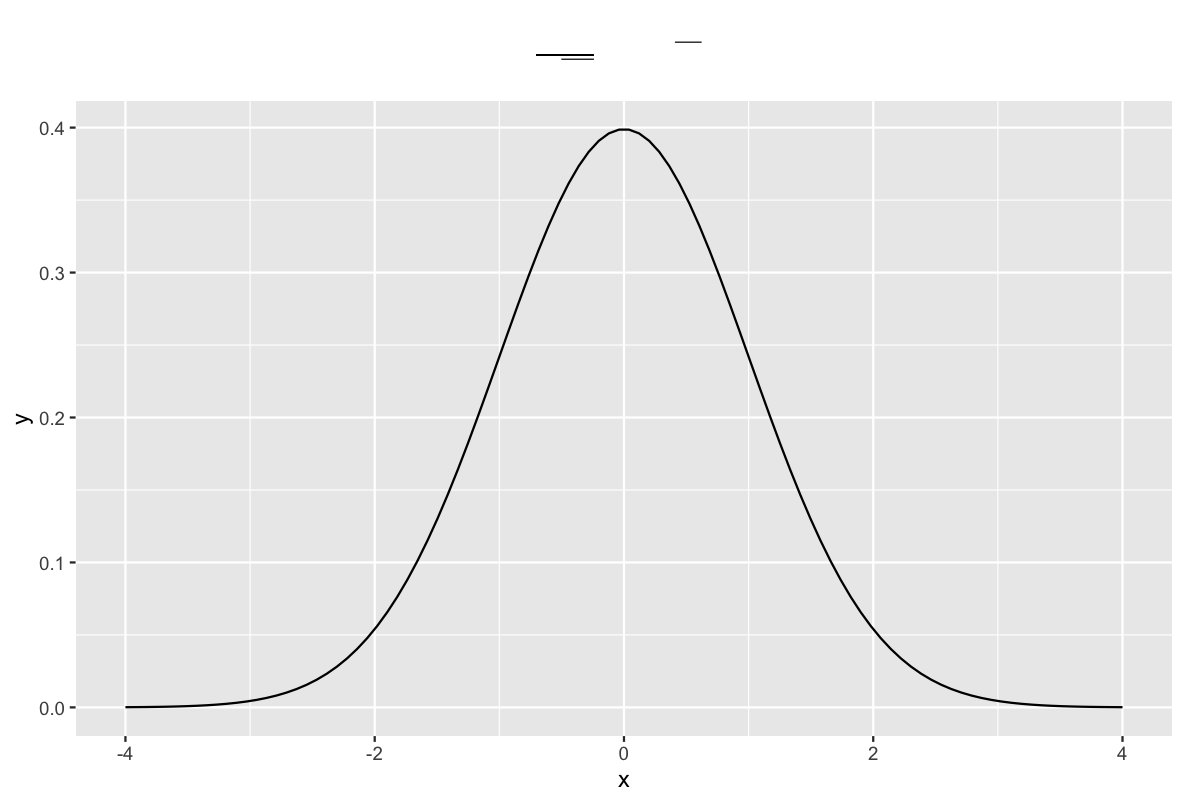
\includegraphics[width=\textwidth]{plot_issue.png}

This was a bug in the glyph-rendering code for the \code{quartz()} graphics 
device.  The bug has been fixed in the development version of R.

\begin{lcverbatim}
  The package contains a `tests` directory, but it appears to not involve a 
  testing framework (e.g. {testthat}). Perhaps these tests are run manually? 
  The test code appears to only check that it runs without error, not that it 
  produces an expected result. I do not see any tests for {ggplot2} generated 
  figures, and no validation that this produces an expected result. Such a test
  may have caught the above issue.
\end{lcverbatim}

I have a large regression test suite (including \textbf{ggplot2} tests)
that makes use of \textbf{gdiff} 
to check for visual differences.
These tests are
not part of the CRAN submission, partly because of the size of the
control images and partly because of the time required to run these tests.

\section*{Response to Editor}

\begin{lcverbatim}
  The LaTeX \color{} command does not take a second argument. It simply changes
  the color from that point onwards. I think you mean \textcolor{}{}.
\end{lcverbatim}

Inappropriate uses of \verb|\color{}| have been changed to 
\verb|\textcolor{}|.

\begin{lcverbatim}
  In Figure 6, please use em-dashes (---) rather than hyphens (-).
\end{lcverbatim}

Hyphens have been replaced with em-dashes in Figure 6.

\begin{lcverbatim}
  You mix plain TeX commands within LaTeX environments. I suggest you replace 
  {\bf ..} with \textbf{..} and {\it ..} with \textit{..}. The results are not 
  identical.
\end{lcverbatim}

Instances of \verb|{\bf ...}| have been replaced with \verb|\textbf{...}|.

\begin{lcverbatim}
  In the discussion, it is perhaps worth including the ggtikz package.
\end{lcverbatim}

The \textbf{ggtikz} package 
is now mentioned in the Discussion, within the paragraph on 
the \textbf{tikzDevice} package [page 22].

\end{document}
